\documentclass[11pt]{article} % Taille globale de texte augmentée
\usepackage{graphicx} % Pour insérer des images
\usepackage[utf8]{inputenc} % Encodage UTF-8
\usepackage[T1]{fontenc} % Fontes adaptées aux accents
\usepackage[french]{babel} % Support du français
\usepackage{amsmath}
\usepackage{amssymb}
\usepackage{pgfplots}
\usepackage{amsthm}  % permet de définir des environnements comme remark
\usepackage{tikz}
\usepackage{tkz-tab}
\newtheorem*{remark}{Remarque:}
\usepackage{amsthm} % Nécessaire pour les environnements de théorèmes
\usepackage{minted}
\usepackage{hyperref}
\usepackage{tkz-tab}


\newtheorem{lemma}{Lemme}




% Titre du document
% Titre du document
\title{
\begin{center}
    
\includegraphics[width=0.9\textwidth]{logo-UT-site.png} \\[1em] % Image ajustée
    {\Huge \textbf{Phénomène de Gibbs}} \\[1em]
    {\Large Projet de la Licence de Mathématiques (L3)} \\\\[0.5em]
    Université de Toulouse
\end{center}
}

\author{
    \textbf{Alexandre MOISE LEUNG} \\
    \textbf{Samiya BENAMMOU} \\
    \textbf{Insafe LAHBICHI} \\
    \textbf{Alison SECLIN}  
}


\date{Printemps 2025}



\usepackage{listings}
\usepackage{xcolor}

\lstset{
  language=Python,
  basicstyle=\ttfamily\small,
  keywordstyle=\color{blue},
  commentstyle=\color{gray},
  stringstyle=\color{orange},
  showstringspaces=false,
  frame=single,
  breaklines=true,
  tabsize=2
}


\begin{document}
\begin{large}

\maketitle


\vspace{0.5cm}
\vfill
\begin{center}
    {\Large \textsc{Encadrante : Rayan Fahs}}
\end{center}
\vspace{1cm}




\newpage
\tableofcontents



\newpage
\section{Introduction}


La représentation des fonctions périodiques au moyen de séries de Fourier constitue un outil fondamental en analyse et en mathématiques appliquées. Introduites par \textit{Joseph Fourier} au début du XIX\textsuperscript{e} siècle, les séries de Fourier permettent d’exprimer une fonction périodique comme une somme infinie de fonctions trigonométriques. Ce procédé trouve de nombreuses applications, notamment en physique, en traitement du signal, en acoustique ou encore en électronique.

Lorsque \( f \) est continue, sa série de Fourier converge uniformément vers \( f \). En revanche, si \( f \) présente des discontinuités, la convergence est seulement ponctuelle, et des oscillations apparaissent près des points de saut. Ce comportement est connu sous le nom de \textbf{phénomène de Gibbs}. Il s'agit d'une limitation dans l’\textit{approximation par séries de Fourier} des fonctions discontinues : au voisinage des discontinuités, la série partielle dépasse systématiquement la valeur cible. \textbf{Le paramètre $N$ désigne ici le nombre de termes considérés dans la somme partielle de la série de Fourier.} Même en augmentant \( N \), ces oscillations ne disparaissent pas. On observe un dépassement qui atteint environ 9\,\% de la hauteur du saut, et ce dépassement persiste quelle que soit la valeur de \( N \).

L’objectif de ce travail est d’étudier rigoureusement le phénomène de Gibbs, tant du point de vue théorique que pratique. Après avoir rappelé les notions fondamentales relatives aux fonctions périodiques et aux séries de Fourier, nous analyserons les conditions de convergence de ces dernières et mettrons en évidence l’apparition des oscillations caractéristiques au voisinage des discontinuités. Nous illustrerons ces phénomènes à l’aide d’exemples concrets et de simulations numériques.




\section{Fonctions périodiques}

\subsection{Définition}

Une fonction \( f : \mathbb{R} \rightarrow \mathbb{R} \) est dite \textbf{périodique} de période \( T > 0 \) si pour tout \( x \in \mathbb{R} \),
\[
f(x + T) = f(x)
\]


\subsection{Exemples classiques}

\begin{itemize}
  \item Les fonctions trigonométriques usuelles telles que \( \sin(x) \) et \( \cos(x) \) sont \( 2\pi \)-périodiques et jouent un rôle central dans le développement des séries de Fourier.

  \item Une autre classe d’exemples intéressants est constituée par les fonctions définies par morceaux, comme la fonction en escalier de Dirichlet. Il s’agit d’une fonction périodique de période \( 2\pi \), définie sur un intervalle fondamental par :

  \[
  f(x) =
  \begin{cases}
  1 & \text{si } x \in [0, \pi], \\
  0 & \text{si } x = 0 \text{ ou } x = \pi, \\
  -1 & \text{si } x \in [-\pi, 0]
  \end{cases}
  \]

  \noindent 
\end{itemize}


\section{Séries de Fourier}

\subsection{Définition}

Soit \( f \) une fonction réelle, périodique de période \( T \), et localement intégrable. Sa \textbf{série de Fourier} est une somme infinie de fonctions trigonométriques (ou exponentielles complexes) permettant de représenter \( f \).

Dans le cas général, la série de Fourier de \( f \) s’écrit :
\[
S_N(f,x) = \sum_{n = -\infty}^{+\infty} {f}(n) e^{2i\pi n x/T},
\]

où les \( {f}(n) \) sont les \textbf{coefficients de Fourier}, définis par :
\[
{f}(n) = \frac{1}{T} \int_{0}^{T} f(x) e^{-2i\pi n x/T} \, dx
\]

\subsection{Développement trigonométrique}


On peut également écrire la série de Fourier sous forme réelle :
\[
f(x) \sim \frac{a_0}{2} + \sum_{n=1}^{\infty} \left( a_n \cos\left(\frac{2\pi n x}{T}\right) + b_n \sin\left(\frac{2\pi n x}{T}\right) \right)
\]
avec les coefficients définis par :
\[
a_0 = \frac{2}{T} \int_0^T f(x)\, dx,
\]
\[
a_n = \frac{2}{T} \int_0^T f(x)\cos\left( \frac{2\pi n x}{T} \right) dx,
\]
\[
b_n = \frac{2}{T} \int_0^T f(x)\sin\left( \frac{2\pi n x}{T} \right) dx
\]

\medskip

Le coefficient \( a_0 \) correspond à la \textit{valeur moyenne} de la fonction \( f \) sur une période. Il est divisé par deux dans le développement car, contrairement aux autres coefficients, il ne provient pas de la combinaison de termes symétriques dans la version complexe de la série de Fourier. Cette convention permet d’assurer une répartition harmonieuse des coefficients dans l’expression réelle.
\]
\paragraph{Exemple:}
Une fonction périodique \( f \) de période \( T = 2\pi \) peut être développée en série de Fourier :

\[
f(x) = \frac{a_0}{2} + \sum_{n=1}^{\infty} \left( a_n \cos\left( nx \right) + b_n \sin\left( nx \right) \right)
\]
avec les coefficients :
\[
a_0 = \frac{1}{\pi} \int_{-\pi}^{\pi} f(x) \, dx,
\]
\[
a_n = \frac{1}{\pi} \int_{-\pi}^{\pi} f(x) \cos(nx) \, dx,
\]
\[
b_n = \frac{1}{\pi} \int_{-\pi}^{\pi} f(x) \sin(nx) \, dx
\]

\subsection{Convergence}

La convergence de la série de Fourier dépend des propriétés de la fonction \( f \) :
\begin{itemize}
  \item Si \( f \) est continue et périodique, la série de Fourier converge \textbf{uniformément} vers \( f \).
  \item Si \( f \) est discontinue mais de variation bornée, la série converge \textbf{ponctuellement} vers la moyenne des limites à gauche et à droite :
  \[
  \lim_{N \to \infty} S_N(f,x_0) = \frac{f(x_0^+) + f(x_0^-)}{2}
  \]
\end{itemize}



\section{Le phénomène de Gibbs}

Lorsque l’on approxime une fonction périodique $f$ présentant une ou plusieurs discontinuités à l’aide de sa série de Fourier, un comportement singulier apparaît au voisinage de ces points de discontinuité. En effet, même si la série converge ponctuellement vers $f(x)$ en tout point, elle ne converge pas uniformément lorsque $f$ présente des sauts.

\subsection{Définition}

Le \textbf{phénomène de Gibbs} désigne l’apparition d’oscillations persistantes de la série de Fourier au voisinage des discontinuités de la fonction. Ces oscillations sont visibles même lorsque le nombre de termes dans la série partielle devient très grand.



\subsection{Formule de l’approximation locale}

Soit $x_0$ un point de discontinuité de $f$. On définit la \textbf{hauteur de la discontinuité} en \( x_0 \) par :
\[
h = \left| f(x_0^-) - f(x_0^+) \right|
\]
La série de Fourier \( S_N(f,x) \) satisfait alors, localement :
\[
S_N(f, x_0 + \varepsilon) \approx \frac{f(x_0^+) + f(x_0^-)}{2} + 0.08949 \cdot h
\]


pour un $\varepsilon$ proche de zéro.

Cela signifie que l’amplitude maximale des oscillations autour du point de saut est environ :
\[
\boxed{ \approx 9\% \text{ de la hauteur du saut} }
\]

\subsection{Formule asymptotique d’amplitude}

D’un point de vue analytique, on peut aussi approximer l’amplitude des oscillations par une formule asymptotique en fonction du nombre de termes $n$ :

\[
\text{Amplitude des oscillations} \approx \frac{1}{2} \cdot \frac{1}{\sqrt{n}}
\]

où $n$ est le rang du dernier terme considéré dans la série. Cette formule montre que bien que l’\textbf{étendue} des oscillations diminue, leur \textbf{amplitude maximale} reste bornée : le phénomène de Gibbs ne disparaît pas.


\section{Exemples}
\subsection{Fonction continue}
Considérons la fonction définie sur l’intervalle \( [-\pi, \pi] \) par :
\[
f(x) = 1 + \sin(x),
\]
et que l’on prolonge en une fonction \( 2\pi \)-périodique sur \( \mathbb{R} \).

Cette fonction est continue, périodique, de classe \( \mathcal{C}^1 \), et donc la série de Fourier converge uniformément vers \( f \) sur \( \mathbb{R} \). 

\subsection*{-> Calcul des coefficients de Fourier}

On cherche à écrire la série de Fourier de \( f \) sous la forme :
\[
f(x) \sim \frac{a_0}{2} + \sum_{n=1}^{\infty} \left( a_n \cos(nx) + b_n \sin(nx) \right)
\]

\paragraph{Coefficient \( a_0 \) :}
\[
a_0 = \frac{1}{\pi} \int_{-\pi}^{\pi} (1 + \sin(x)) \, dx = \frac{1}{\pi} \left( \int_{-\pi}^{\pi} 1 \, dx + \int_{-\pi}^{\pi} \sin(x) \, dx \right) = \frac{1}{\pi} (2\pi + 0) = 2
\]
Donc \( \frac{a_0}{2} = 1 \)

\paragraph{Coefficients \( a_n \) :}
\[
a_n = \frac{1}{\pi} \int_{-\pi}^{\pi} (1 + \sin(x)) \cos(nx) \, dx  \left = \frac{1}{\pi} \int_{-\pi}^{\pi} \cos(nx) + \sin(x) \cos(nx) dx\right 
\]
Calculons l'intégrale suivante :
\[
\int_{-\pi}^{\pi} \cos(nx) \, dx
\]

On utilise une primitive de \(\cos(nx)\), qui est :
\[
\int \cos(nx) \, dx = \frac{\sin(nx)}{n}
\]

Ainsi,
\[
\int_{-\pi}^{\pi} \cos(nx) \, dx = \left[ \frac{\sin(nx)}{n} \right]_{-\pi}^{\pi} = \frac{1}{n} \left( \sin(n\pi) - \sin(-n\pi) \right)
\]

Or, pour tout entier \( n \), on sait que :
\[
\sin(n\pi) = 0 \quad \text{et} \quad \sin(-n\pi) = 0
\]

Donc :
\[
\int_{-\pi}^{\pi} \cos(nx) \, dx = \frac{1}{n} (0 - 0) = 0
\]
De plus :
 \quad
\int_{-\pi}^{\pi} \sin(x) \cos(nx) \, dx = 0,


Car pour tout entier \( n \geq 1 \), on observe que \( \sin(x) \) est une fonction impaire, c’est-à-dire que \( \sin(-x) = -\sin(x) \), tandis que \( \cos(nx) \) est paire, donc \( \cos(-nx) = \cos(nx) \).

Le produit \( \sin(x) \cos(nx) \) est donc une fonction impaire, car :
\[
[\sin(x)\cos(nx)](-x) = \sin(-x)\cos(-nx) = -\sin(x)\cos(nx)
\]
Or, l’intégrale d’une fonction impaire sur un intervalle symétrique centré en zéro, comme \( [-\pi, \pi] \), est toujours nulle. Ainsi :
\[
\int_{-\pi}^{\pi} \sin(x) \cos(nx) \, dx = 0
\]

donc \( a_n = 0 \) pour tout \( n \geq 1 \).

\paragraph{Coefficients \( b_n \) :}
\[
b_n = \frac{1}{\pi} \int_{-\pi}^{\pi} (1 + \sin(x)) \sin(nx) \, dx = \frac{1}{\pi} \left( \int_{-\pi}^{\pi} \sin(nx) \, dx + \int_{-\pi}^{\pi} \sin(x) \sin(nx) \, dx \right)
\]
\[
\int_{-\pi}^{\pi} \sin(nx) \, dx = 0
\]
Pour \( n = 1 \) :
\[
\int_{-\pi}^{\pi} \sin(x) \sin(x) \, dx = \int_{-\pi}^{\pi} \sin^2(x) \, dx = \pi,
\quad \Rightarrow \quad b_1 = \frac{1}{\pi} \cdot \pi = 1
\]
\begin{remark}
Pour évaluer l’intégrale
\[
\int_{-\pi}^{\pi} \sin^2(x) \, dx
\]
on utilise l'identité trigonométrique classique :
\[
\sin^2(x) = \frac{1 - \cos(2x)}{2}
\]
On a alors :
\[
\int_{-\pi}^{\pi} \sin^2(x) \, dx = \int_{-\pi}^{\pi} \frac{1 - \cos(2x)}{2} \, dx = \frac{1}{2} \int_{-\pi}^{\pi} \left( 1 - \cos(2x) \right) dx
\]

Or,
\[
\int_{-\pi}^{\pi} 1 \, dx = 2\pi, \quad \text{et} \quad \int_{-\pi}^{\pi} \cos(2x) \, dx = 0
\]
car \( \cos(2x) \) est une fonction paire de période \( \pi \) dont l’intégrale sur une période complète centrée en zéro s’annule.

Par conséquent :
\[
\int_{-\pi}^{\pi} \sin^2(x) \, dx = \frac{1}{2} \cdot (2\pi - 0) = \pi
\]
\end{remark}

Pour \( n \neq 1 \), \( \int_{-\pi}^{\pi} \sin(x) \sin(nx) \, dx = 0 \) par orthogonalité.
\begin{remark}
Pour tout entier \( n \neq 1 \), on a :
\[
\int_{-\pi}^{\pi} \sin(x)\sin(nx) \, dx = 0
\]
Cela s’explique par le fait que les fonctions \( \sin(nx) \), pour \( n \in \mathbb{N}^* \), forment une famille orthogonale sur l’intervalle \( [-\pi, \pi] \), c’est-à-dire que :
\[
\int_{-\pi}^{\pi} \sin(mx) \sin(nx) \, dx =
\begin{cases}
0 & \text{si } m \ne n \\
\pi & \text{si } m = n
\end{cases}
\]
Ainsi, les fonctions \( \sin(x) \) et \( \sin(nx) \) sont orthogonales pour \( n \ne 1 \), ce qui justifie l'annulation de l’intégrale.
\end{remark}


Donc \( b_n = \begin{cases} 1 & \text{si } n = 1 \\ 0 & \text{sinon} \end{cases} \)

\subsection*{ -> Série de Fourier de \( f \)}

On obtient :
\[
f(x) = 1 + \sin(x) \sim \frac{a_0}{2} + b_1 \sin(x) = 1 + \sin(x)
\]

La série de Fourier est donc égale à la fonction elle-même et converge uniformément sur \( \mathbb{R} \). Cette convergence est conforme au théorème de convergence uniforme des séries de Fourier pour les fonctions continues et lipschitziennes.


\textbf{Code utilisé } : \hyperref[annexe_code_continue]{voir annexe}

\begin{figure}[h!]
    \centering
    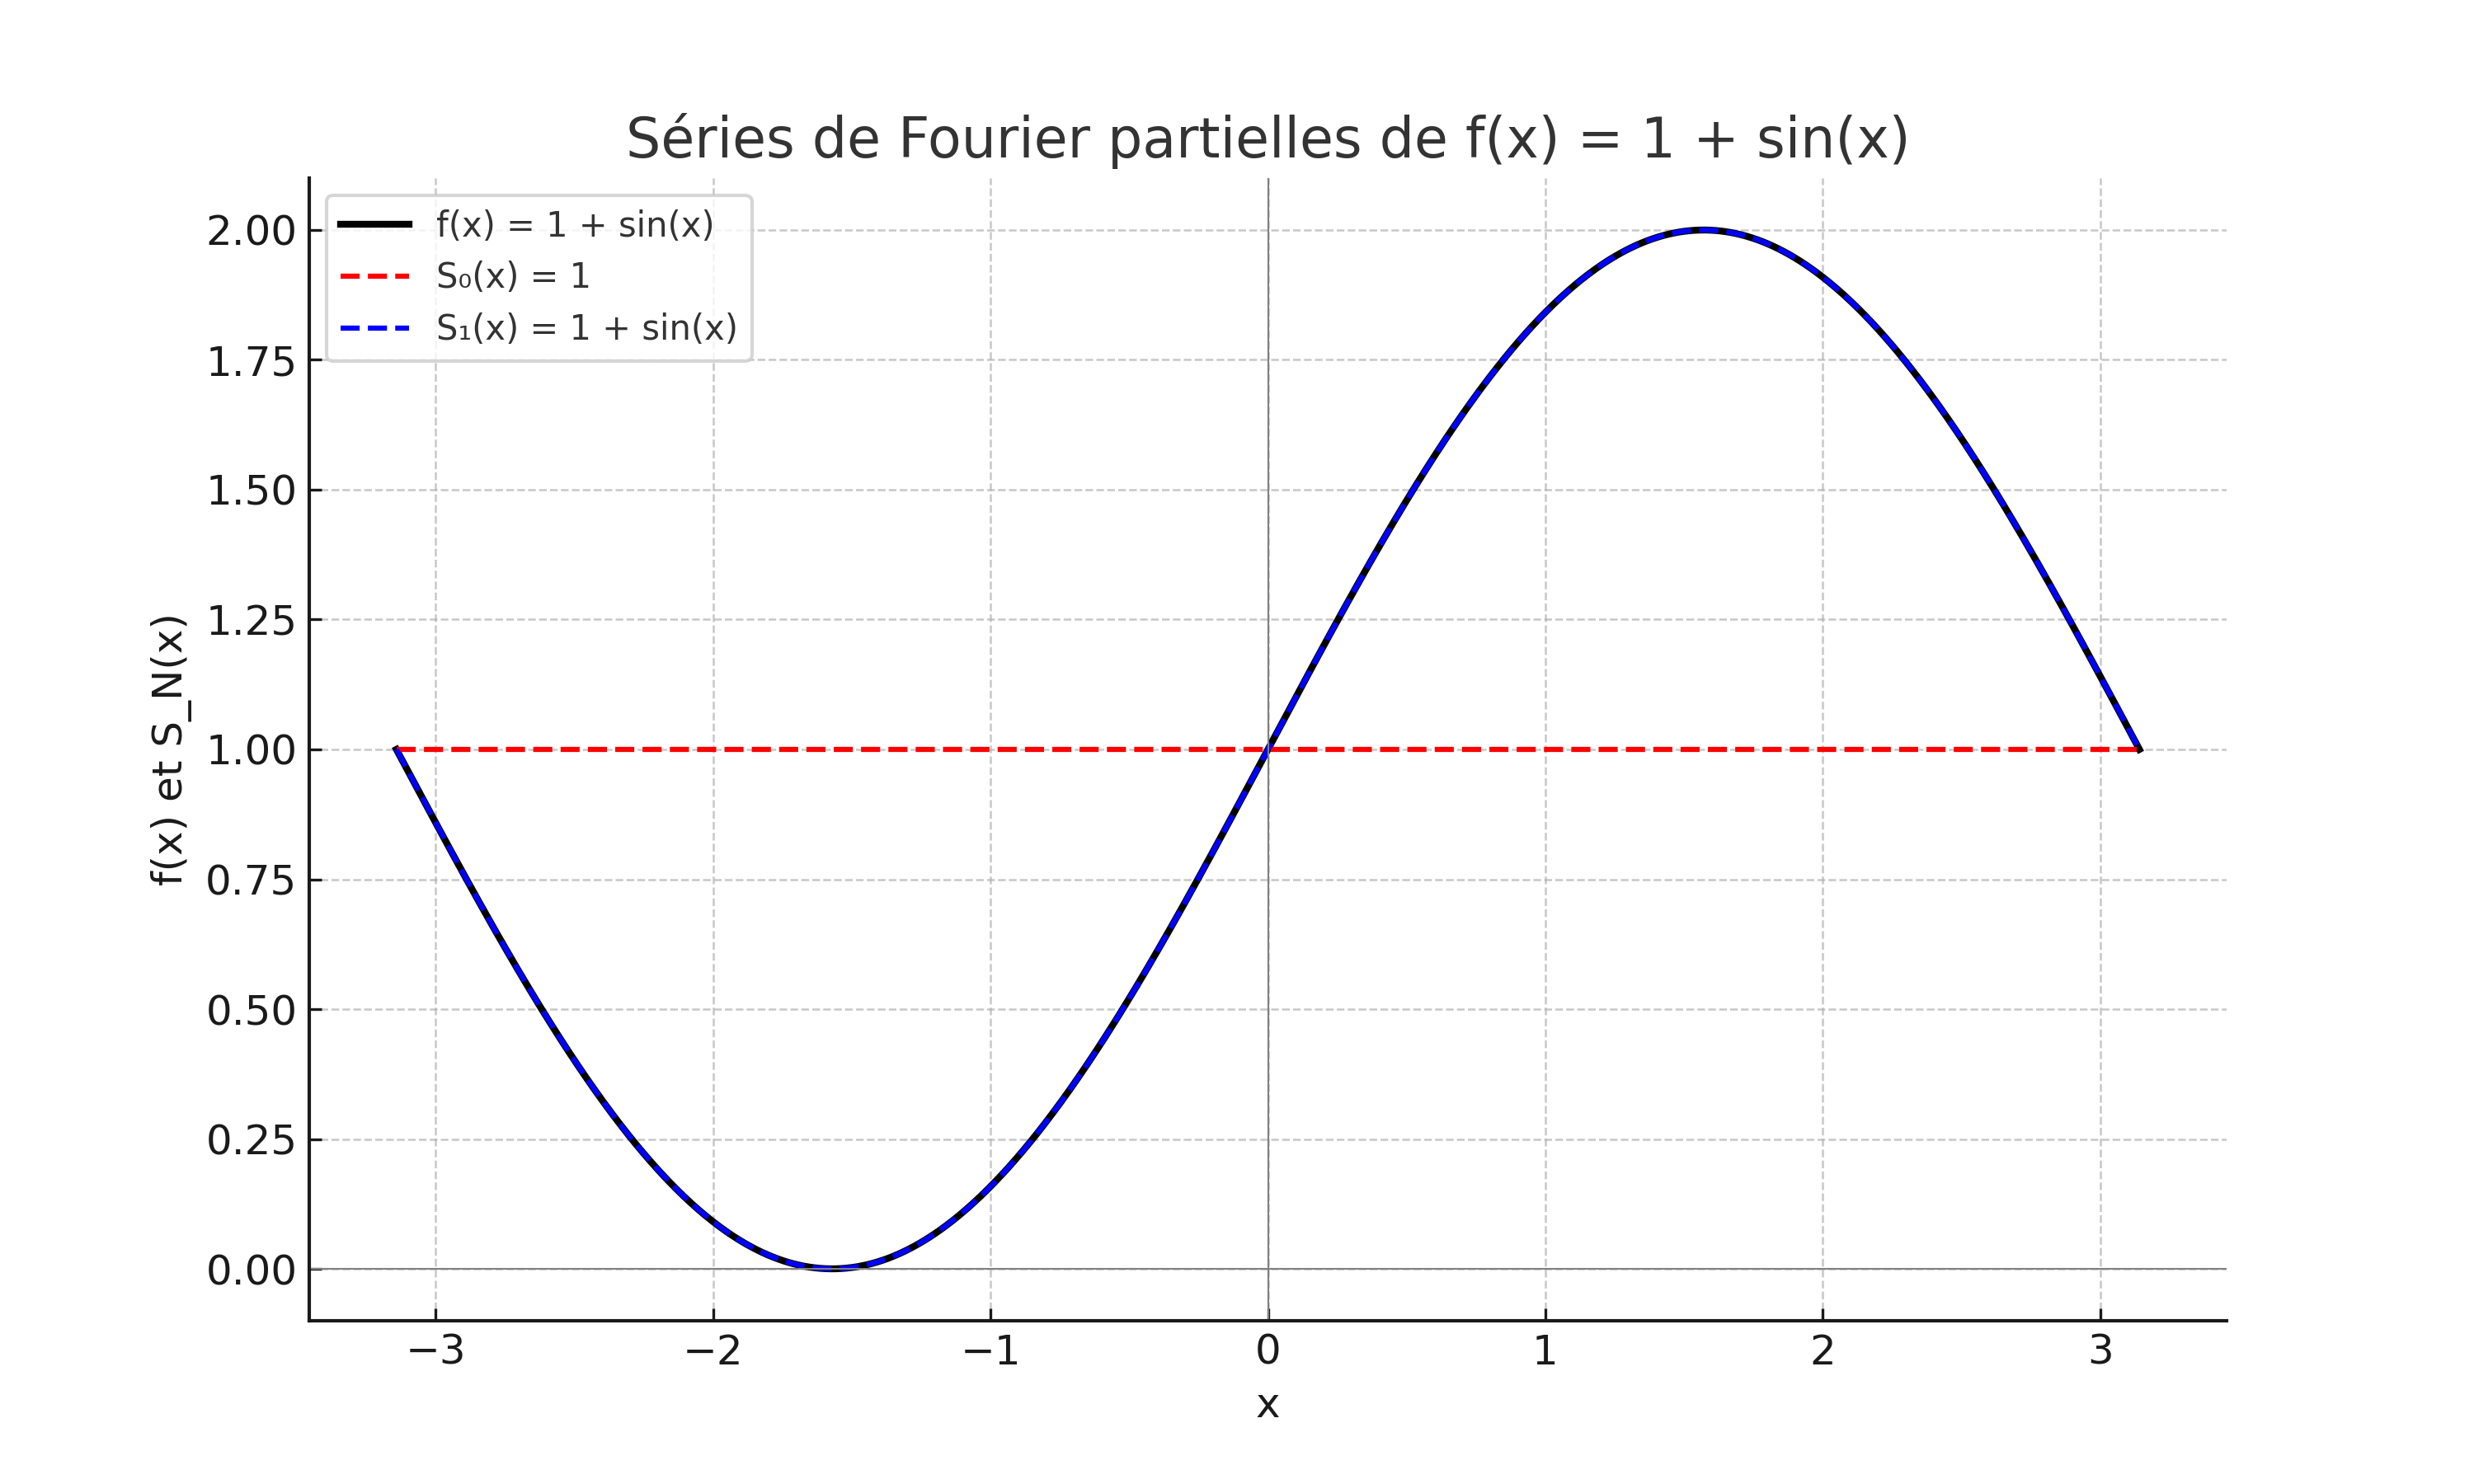
\includegraphics[width=0.8\textwidth]{fourier_sin_graph.png}
    \caption{Série de Fourier partielle de la fonction $f(x) = 1 + \sin(x)$ pour $N = 0$ et $N = 1$.}
    \label{fig:fourier_sin}
\end{figure}



\subsection{Fonction discontinue}

On considère la fonction \( f \), définie par :
\[
f(x) =
\begin{cases}
1 & \text{si } |x| < \frac{\pi}{2} \\
0 & \text{si } \frac{\pi}{2} \leq |x| \leq \pi
\end{cases}
\quad \text{et prolongée par } f(x + 2\pi) = f(x) \text{ pour tout } x \in \mathbb{R}.
\]

\subsection*{-> Parité et période}

La fonction \( f \) est \textbf{paire} : \( f(-x) = f(x) \), donc tous les coefficients \( b_n \) de la série de Fourier sont nuls.  
Elle est \textbf{2π-périodique}, donc on utilise le développement suivant :
\[
f(x) = \frac{a_0}{2} + \sum_{n=1}^\infty a_n \cos(nx)
\]

\subsection*{-> Calcul des coefficients de Fourier}

\paragraph{Coefficient constant :}
\[
a_0 = \frac{1}{\pi} \int_{-\pi}^{\pi} f(x) dx = \frac{2}{\pi} \int_0^{\pi/2} 1 \, dx = \frac{2}{\pi} \cdot \frac{\pi}{2} = 1
\]

\paragraph{Pour \( n \geq 1 \), coefficients \( a_n \) :}
\[
a_n = \frac{1}{\pi} \int_{-\pi}^{\pi} f(x)\cos(nx) dx = \frac{2}{\pi} \int_0^{\pi/2} \cos(nx)\, dx
= \frac{2}{n\pi} \sin\left( \frac{n\pi}{2} \right)
\]

\subsection*{-> Série de Fourier de \( f \)}

On en déduit le développement suivant :
\[
f(x) = \frac{1}{2} + \sum_{n=1}^\infty \frac{2}{n\pi} \sin\left( \frac{n\pi}{2} \right) \cos(nx)
\]

Comme \( \sin(n\pi/2) = 0 \) si \( n \) est pair, on a :
\[
f(x) = \frac{1}{2} + \sum_{k=0}^\infty \frac{2}{(2k+1)\pi} (-1)^k \cos((2k+1)x)
\]


La fonction \( f \) présente des discontinuités en \( x = \pm \frac{\pi}{2}, \pm \frac{3\pi}{2}, \dots \).  
Au voisinage de ces points, les sommes partielles de la série présentent un dépassement de la valeur maximale : c’est le \textbf{phénomène de Gibbs}. Ce dépassement ne disparaît pas quand \( n \to \infty \).


\section*{-> Visualisation des sommes partielles }

Nous présentons ci-dessous les graphes des sommes partielles \( S_N(x) \) de la série de Fourier de la fonction porte pour différentes valeurs de \( N \).

\begin{figure}[h]
    \centering
    \begin{minipage}{0.48\textwidth}
        \centering
        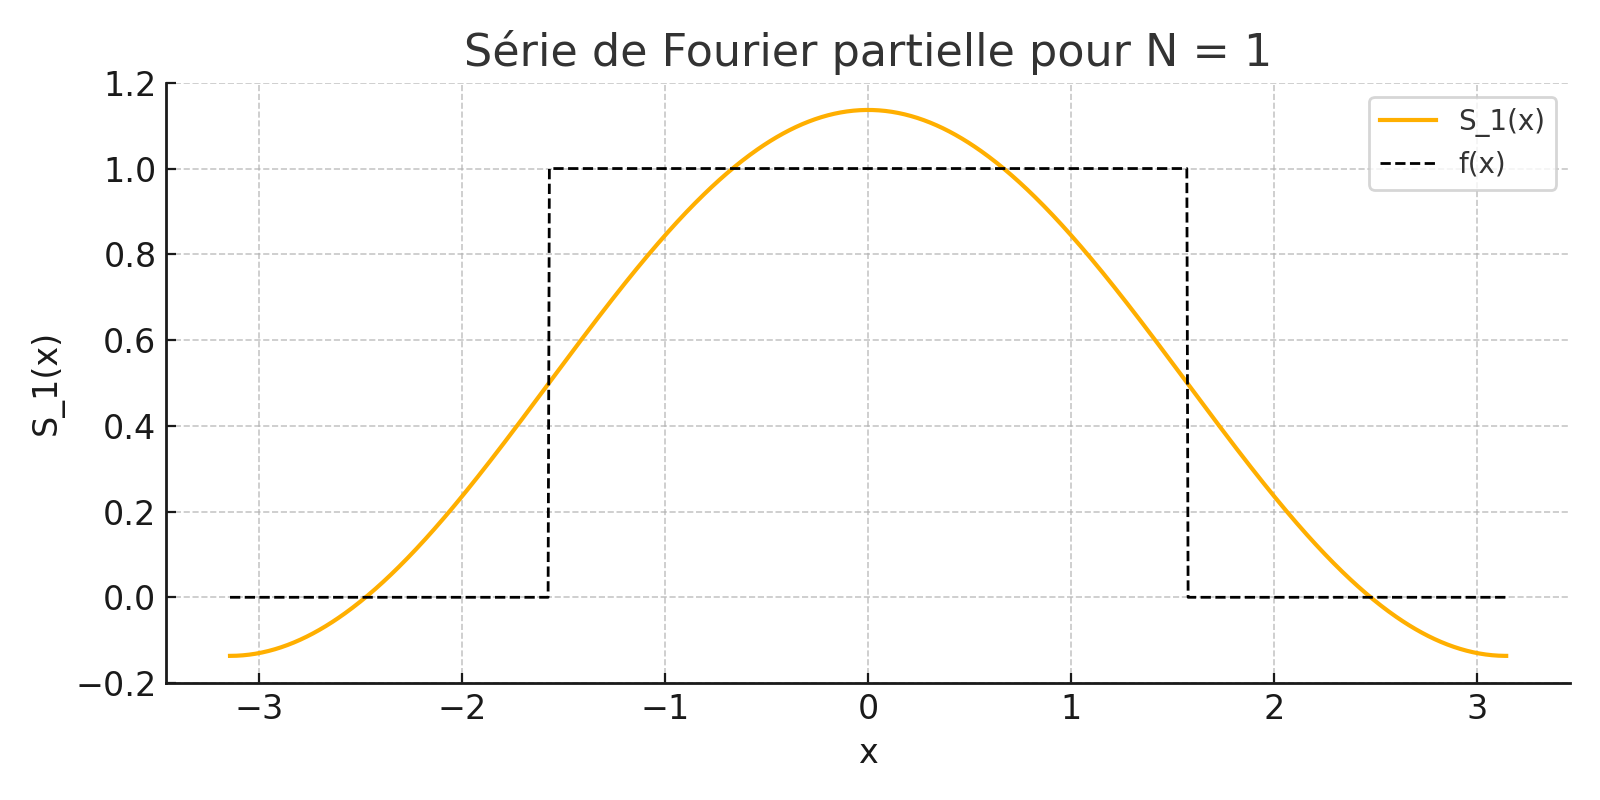
\includegraphics[width=\linewidth]{serie_fourier_N1.png}
        \caption{Somme partielle \( S_1(x) \)}
        \label{fig:S1}
    \end{minipage}
    \hfill
    \begin{minipage}{0.48\textwidth}
        \centering
        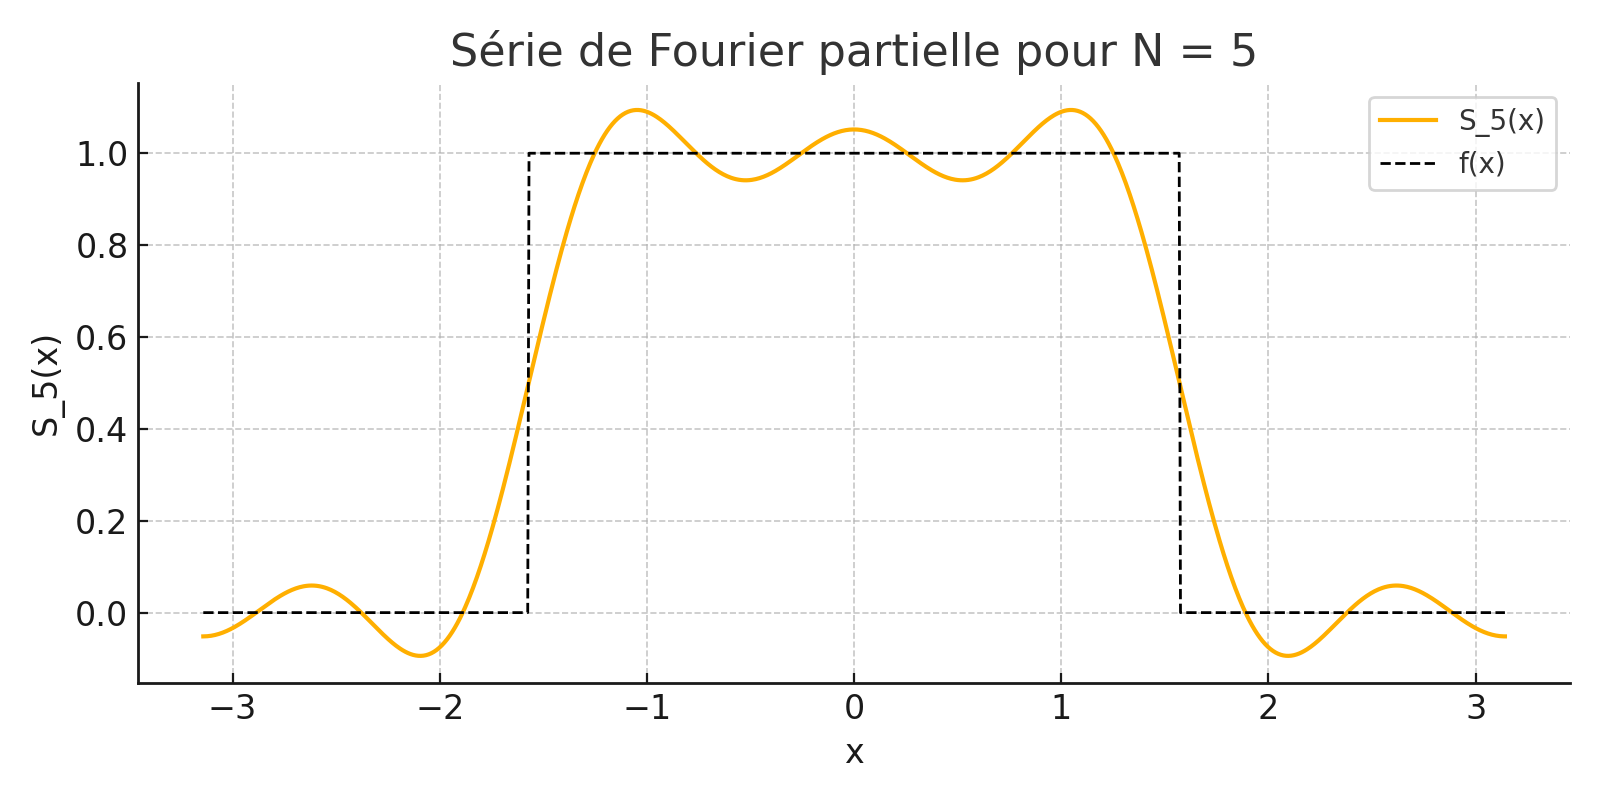
\includegraphics[width=\linewidth]{serie_fourier_N5.png}
        \caption{Somme partielle \( S_5(x) \)}
        \label{fig:S5}
    \end{minipage}
\end{figure}


\begin{figure}[h]
    \centering
    \begin{minipage}{0.48\textwidth}
        \centering
        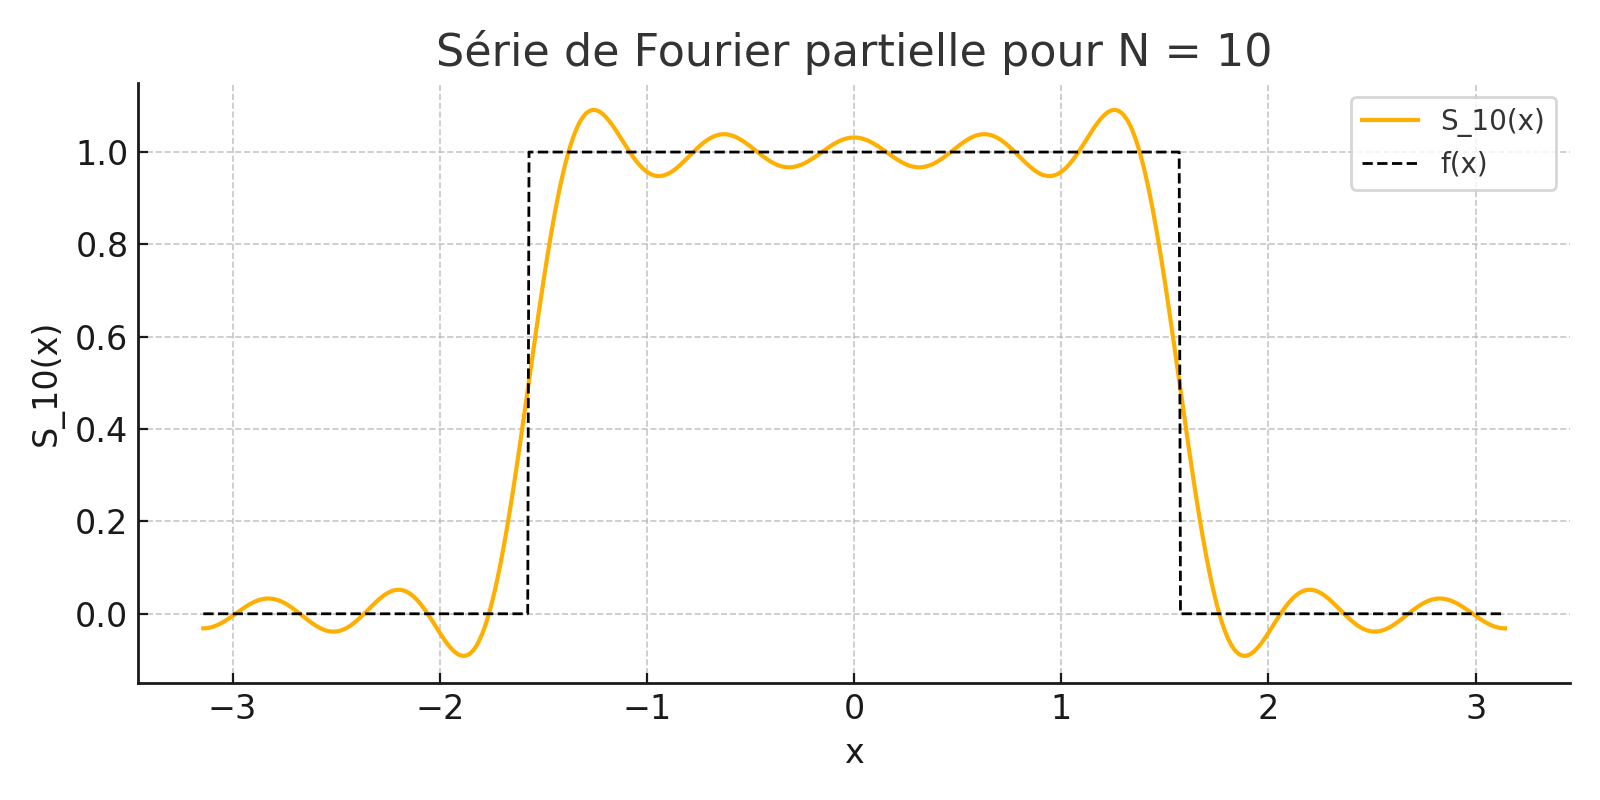
\includegraphics[width=\linewidth]{serie_fourier_N10.png}
        \caption{Somme partielle \( S_{10}(x) \)}
        \label{fig:S10}
    \end{minipage}
    \hfill
    \begin{minipage}{0.48\textwidth}
        \centering
        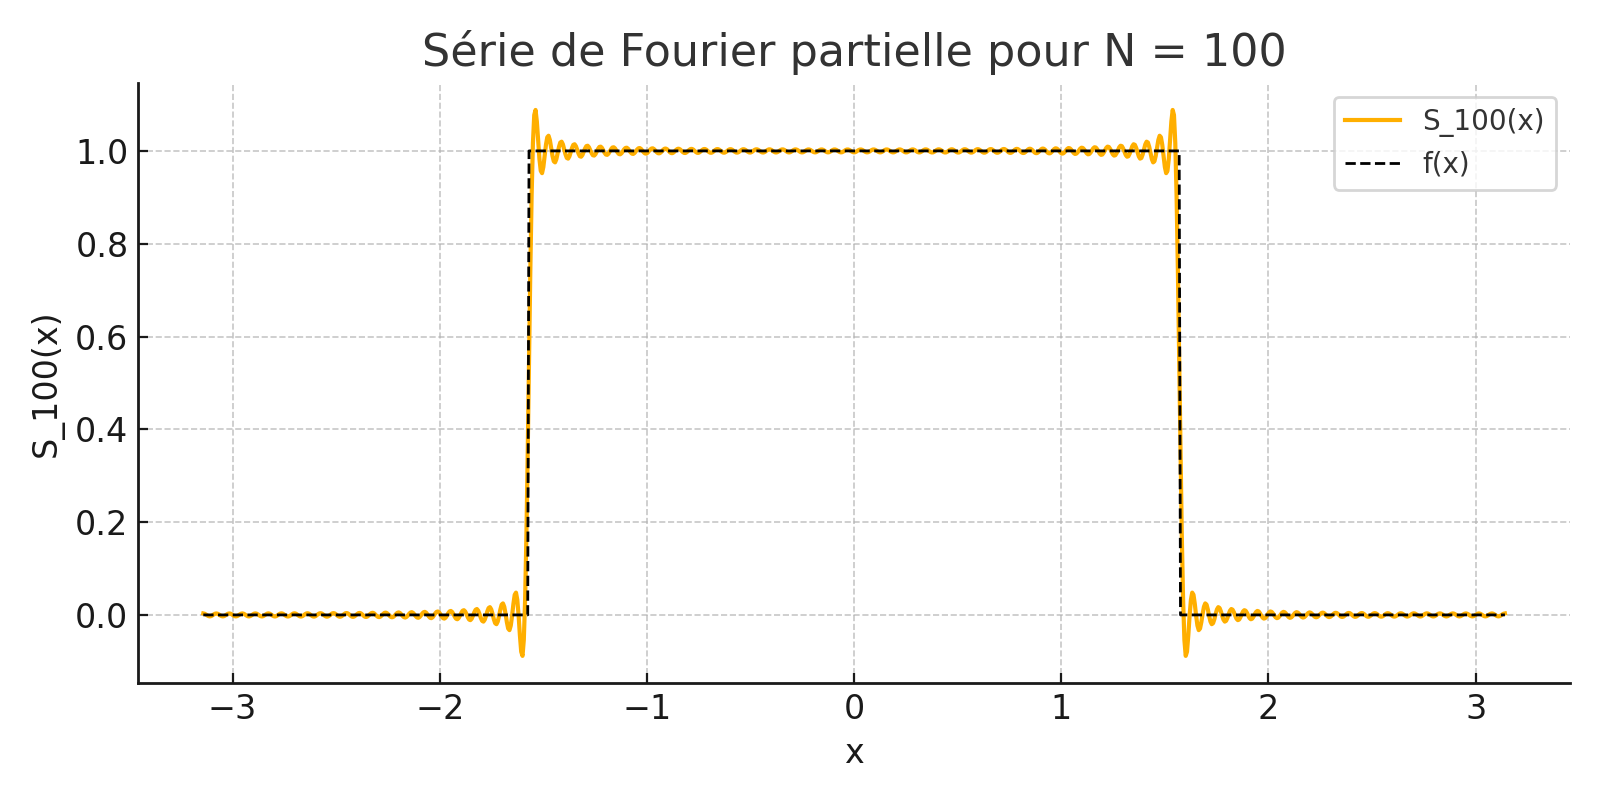
\includegraphics[width=\linewidth]{serie_fourier_N100.png}
        \caption{Somme partielle \( S_{100}(x) \) }
        \label{fig:S100}
    \end{minipage}
\end{figure}

\vspace{0.5em}
\noindent\textbf{Code utilisé} : \hyperref[annexe_code_python]{voir annexe}



\section*{-> Interprétation des résultats}


Les figures représentant les sommes partielles \( S_N(x) \) de la série de Fourier de la fonction porte montrent une évolution nette du comportement des approximations de \( f(x) \) lorsque le nombre de termes \( N \) augmente :

\begin{itemize}
  \item Pour \( N = 1 \), l’approximation est très grossière 
  
  \item Pour \( N = 5 \), la forme globale du signal rectangulaire commence à apparaître, mais de fortes oscillations sont visibles à proximité des discontinuités en \( x = \pm \frac{\pi}{2} \).
  
  \item Pour \( N = 10 \), l’approximation s’améliore nettement dans les zones continues, mais les oscillations deviennent plus prononcées près des discontinuités. C’est la manifestation du \textbf{phénomène de Gibbs}.
  
  \item Pour \( N = 100 \), la série de Fourier est très proche de la fonction exacte en dehors des discontinuités, mais on observe un \textbf{dépassement constant et localisé} autour de \( x = \pm \frac{\pi}{2} \), dont l’amplitude ne disparaît pas avec \( N \). Ce dépassement est d’environ 9\% de la hauteur du saut.
\end{itemize}

Ces observations illustrent parfaitement le \textbf{phénomène de Gibbs}, selon lequel les séries de Fourier approchent bien les fonctions continues, mais présentent des dépassements au voisinage des discontinuités, indépendamment de la valeur de \( N \).












\newpage

\section{Étude théorique du phénomène de Gibbs}


Dans cette section, nous allons mettre en évidence le phénomène de Gibbs à travers l'étude mathématique rigoureuse de la série de Fourier d'une fonction \( f \) impaire et \( 2\pi \)-périodique, définie par :

\[
f(x) =
\begin{cases}
1 & \text{si } x \in ]0, \pi[ \\
-1 & \text{si } x \in ]-\pi, 0[ \\
0 & \text{si } x = 0, \pi
\end{cases}
\]

Cette fonction présente une discontinuité en \( x = 0 \) et \( x = \pi \), ce qui en fait un exemple parfait pour illustrer le dépassement de Gibbs.

Nous allons d'abord déterminer les coefficients de Fourier de \( f \), puis analyser la convergence de sa série, calculer les sommes partielles et leurs dérivées, et enfin étudier le comportement local autour de \( t = 0 \), où le phénomène de Gibbs se manifeste.




\subsection{Calcul des coefficients de Fourier}

La fonction étant impaire, sa série de Fourier ne contient que des termes en sinus :
\[
b_n = \frac{1}{\pi} \int_{-\pi}^{\pi} f(x) \sin(nx) \, dx
= \frac{2}{\pi} \int_0^{\pi} f(x) \sin(nx) \, dx
= \frac{2}{\pi} \int_0^{\pi} \sin(nx) \, dx
\]

\[
= \frac{2}{\pi} \left[ -\frac{\cos(nx)}{n} \right]_0^\pi
= \frac{2}{\pi n} (1 - (-1)^n)
=
\begin{cases}
\frac{4}{\pi n} & \text{si } n \text{ impair} \\
0 & \text{si } n \text{ pair}
\end{cases}
\]

\subsection{Développement en série de Fourier}

On en déduit que sa série de Fourier s'écrit :
\[
f(x) = \sum_{\substack{n=1 \\ n \text{ impair}}}^{\infty} \frac{4}{\pi n} \sin(nx)
= \frac{4}{\pi} \sum_{k=1}^\infty \frac{\sin((2k-1)x)}{2k - 1}
\quad \text{pour tout } x \in ]0, \pi[.
\]
 


En particulier, pour tout $t \in ]0, \pi[$, on a $f(t) = 1$, donc :
\[
1 = \frac{4}{\pi} \sum_{k=1}^{\infty} \frac{\sin((2k - 1)t)}{2k - 1}
\]

En t = 0, on a f(0) = 0,
donc:
\[
\sum_{k=1}^{\infty} \frac{\sin((2k - 1) \cdot 0)}{2k - 1} = 0
\]


\subsection{Calcul de la dérivée de $S_p(t)$}



On considère la somme partielle de la série de Fourier :
\[
S_p(t) = \frac{4}{\pi} \sum_{k=1}^{p} \frac{\sin((2k - 1)t)}{2k - 1}
\]

La dérivation terme à terme est permise car la somme est finie. La dérivée d'un sinus est donnée par :
\[
\frac{d}{dt}[\sin((2k - 1)t)] = (2k - 1)\cos((2k - 1)t)
\]
Ainsi, la dérivée de $S_p(t)$ est :
\[
S_p'(t) = \frac{4}{\pi} \sum_{k=1}^{p} \cos((2k - 1)t)
\]

On reconnaît ici une somme de cosinus. On peut exprimer chaque terme $\cos((2k - 1)t)$ comme la partie réelle de $e^{i(2k - 1)t}$ :
\[
\cos((2k - 1)t) = \Re\left(e^{i(2k - 1)t}\right)
\]
donc :
\[
S_p'(t) = \frac{4}{\pi} \Re\left( \sum_{k=1}^{p} e^{i(2k - 1)t} \right)
\]

Cette somme est une suite géométrique de premier terme $e^{it}$ et de raison $e^{2it}$ :

\begin{align*}
\sum_{k=1}^{p} e^{i(2k-1)t}
&= e^{it} + e^{i3t} + \dots + e^{i(2p - 1)t} \\
&= e^{it} \left(1 + e^{i2t} + e^{i4t} + \dots + e^{i2(p - 1)t} \right) \\
&= e^{it} \sum_{k=0}^{p - 1} (e^{i2t})^k \\
&= e^{it} \cdot \frac{1 - e^{i2pt}}{1 - e^{i2t}}
\end{align*}





En utilisant la relation :
\[
\frac{1 - e^{2ipt}}{1 - e^{2it}} = \frac{e^{ipt} \cdot (e^{-ipt} - e^{ipt})}{e^{it} \cdot (e^{-it} - e^{it})} = e^{i(p - 1)t} \cdot \frac{\sin(pt)}{\sin(t)}
\]

on obtient :
\[
S_p'(t) = \frac{4}{\pi} \Re\left( e^{ipt} \cdot \frac{\sin(pt)}{\sin(t)} \right)
= \frac{4}{\pi} \cdot \cos(pt) \cdot \frac{\sin(pt)}{\sin(t)}
\]

En utilisant l'identité trigonométrique $\sin(2pt) = 2\sin(pt)\cos(pt)$, on trouve finalement :
\[
S_p'(t) = \frac{2}{\pi} \cdot \frac{\sin(2pt)}{\sin(t)}
\]

C'est l'expression finale de la dérivée de la somme partielle \( S_p(t) \).


\subsection{Forme intégrale de $S_p(t)$}

On a démontré précédemment que :
\[
S'_p(t) = \frac{2}{\pi} \cdot \frac{\sin(2pt)}{\sin(t)}
\]

En intégrant cette expression entre 0 et \( t \), et en utilisant le fait que \( S_p(0) = 0 \), on obtient :
\[
S_p(t) = \int_0^t S'_p(u) \, du
= \frac{2}{\pi} \int_0^t \frac{\sin(2pu)}{\sin(u)} \, du
\]

Cette expression intégrale sera utilisée dans l'étude asymptotique du comportement de \( S_p(t) \) au voisinage des discontinuités.






\subsection{Étude de la dérivée de \( S_p(t) \) et maximum local}

On a montré précédemment que la dérivée de la somme partielle est donnée par :
\[
S_p'(t) = \frac{2}{\pi} \cdot \frac{\sin(2pt)}{\sin t}
\]

Sur l'intervalle \( t \in ]0, \pi[ \), on a \( \sin t > 0 \), donc le signe de \( S_p'(t) \) dépend uniquement de \( \sin(2pt) \).

On a : 
\[
S_p'(t) = 0 \quad \Leftrightarrow \quad \sin(2pt) = 0 \quad \Leftrightarrow \quad t = \frac{k\pi}{2p} , \quad \text{avec } k \in \mathbb{Z}
\]

Le premier zéro non nul est atteint pour \( t = \frac{\pi}{2p} \).  
On étudie le signe de la dérivée de part et d’autre :

\begin{itemize}
  \item Sur \( ]0, \frac{\pi}{2p}[ \), on a \( \sin(2pt) > 0 \Rightarrow S_p'(t) > 0 \)
  \item Sur \( ]\frac{\pi}{2p}, \frac{\pi}{p}[ \), on a \( \sin(2pt) < 0 \Rightarrow S_p'(t) < 0 \)
\end{itemize}

\paragraph{Tableau de variation de \( S_p \) sur \( [0, \frac{\pi}{p}] \) :}

\begin{center}
\begin{tikzpicture}
  \tkzTabInit[lgt=2.5, espcl=4]%
  {$t$ /1, $S_p'(t)$ /1, $S_p(t)$ /2}%
  {$0$, $\dfrac{\pi}{2p}$, $\dfrac{\pi}{p}$}
  \tkzTabLine{,+,z,-}
  \tkzTabVar{-/ , +/ $\text{max local}$ , -/ }
\end{tikzpicture}
\end{center}


Donc:

\[
m_{1,p} = S_p\left( \frac{\pi}{2p} \right)
= \frac{2}{\pi} \int_0^{\frac{\pi}{2p}} \frac{\sin(2pu)}{\sin u} \, du
\]









\subsection{Passage à la limite et phénomène de Gibbs}

On a montré que :
\[
m_{1,p} = \frac{2}{\pi} \int_0^{\gamma_p} \frac{\sin y}{\sin\left( \frac{y}{2p} \right)} \cdot \frac{dy}{2p}
\quad \text{et en posant } \frac{y}{2p} = u
\]
on obtient par passage à la limite :
\[
\lim_{p \to \infty} m_{1,p} = \frac{2}{\pi} \int_0^{\pi} \frac{\sin y}{y} \, dy \approx 1.179
\]

Cela signifie que :
\[
\sup_{t \in [0, \pi]} |S_p(t) - f(t)| \geq m_{1,p} - 1 \not\to 0
\quad \text{quand } p \to \infty
\]

Ainsi, les séries partielles \( S_p(t) \) \textbf{dépassent toujours} la valeur de la fonction \( f(t) \) au voisinage de \( t = 0 \), et ce dépassement ne disparaît jamais.

\paragraph{Conclusion:}
Ce comportement caractérise le \textbf{phénomène de Gibbs} :\\
la série de Fourier, bien que convergente ponctuellement, ne converge pas uniformément lorsque la fonction possède des discontinuités.\\
Le dépassement de l’ordre de 9\,\% persiste, quelle que soit la valeur de \( p \).

\begin{figure}[h]
\centering
\begin{minipage}{0.48\textwidth}
    \centering
    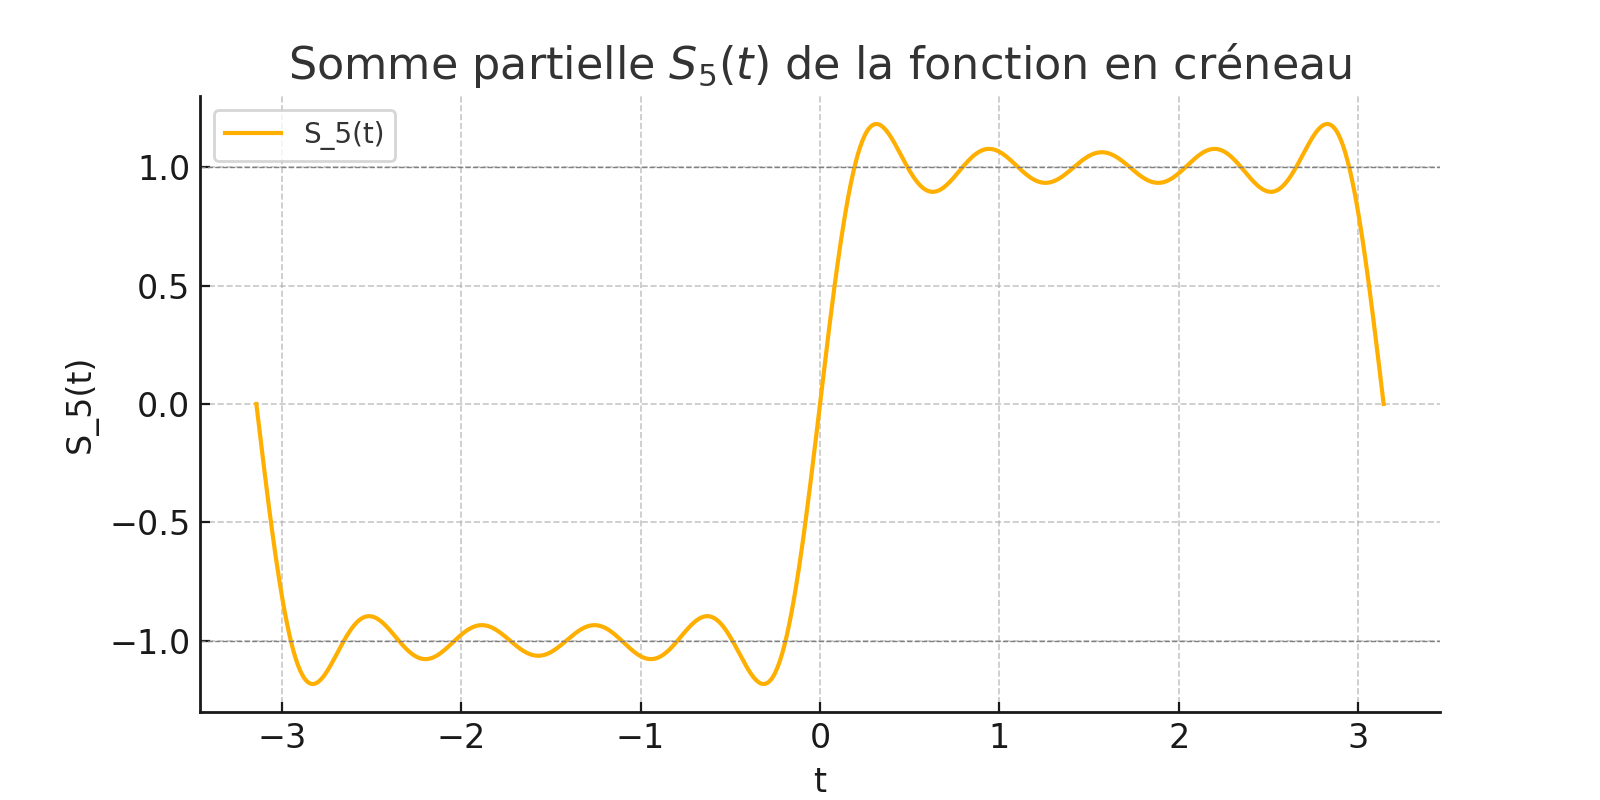
\includegraphics[width=\linewidth]{S_p_t_5.png}
    \caption{Somme partielle \( S_5(t) \)}
\end{minipage}
\hfill
\begin{minipage}{0.48\textwidth}
    \centering
    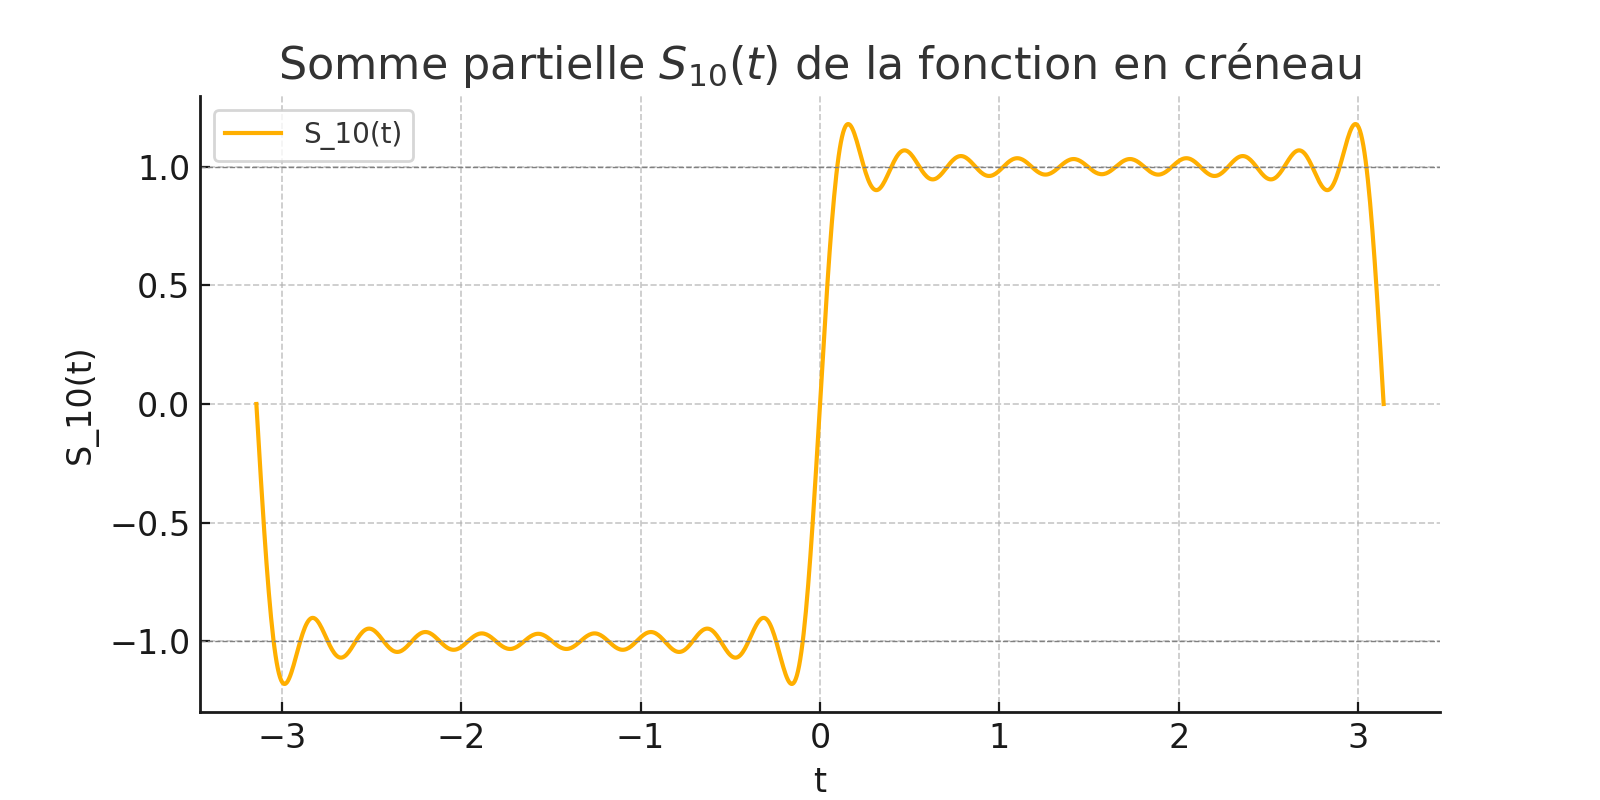
\includegraphics[width=\linewidth]{S_p_t_10.png}
    \caption{Somme partielle \( S_{10}(t) \)}
\end{minipage}
\end{figure}

\begin{figure}[h]
\centering
\begin{minipage}{0.48\textwidth}
    \centering
    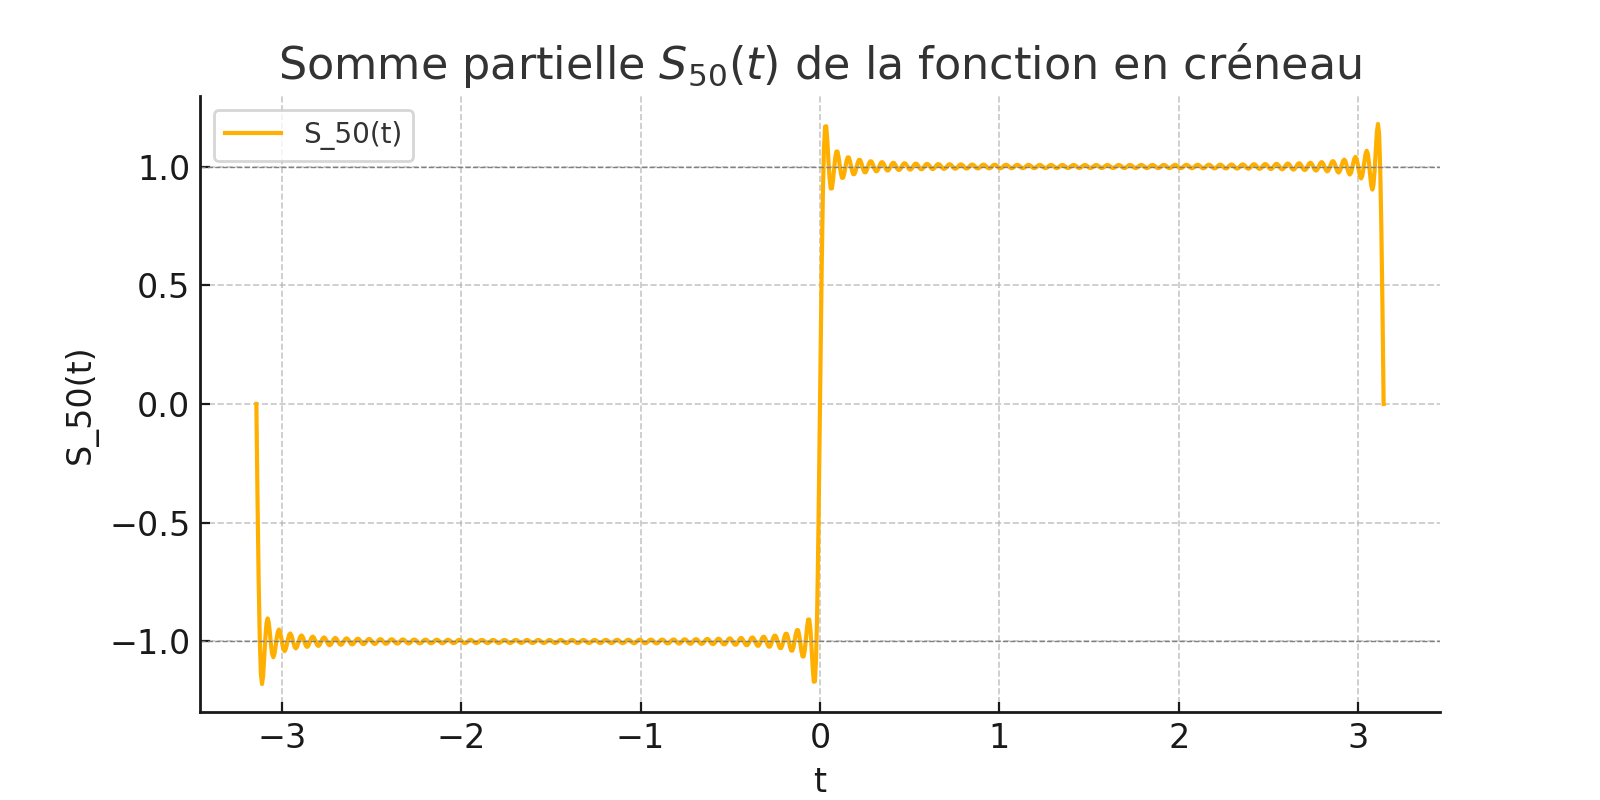
\includegraphics[width=\linewidth]{S_p_t_50.png}
    \caption{Somme partielle \( S_{50}(t) \)}
\end{minipage}
\hfill
\begin{minipage}{0.48\textwidth}
    \centering
    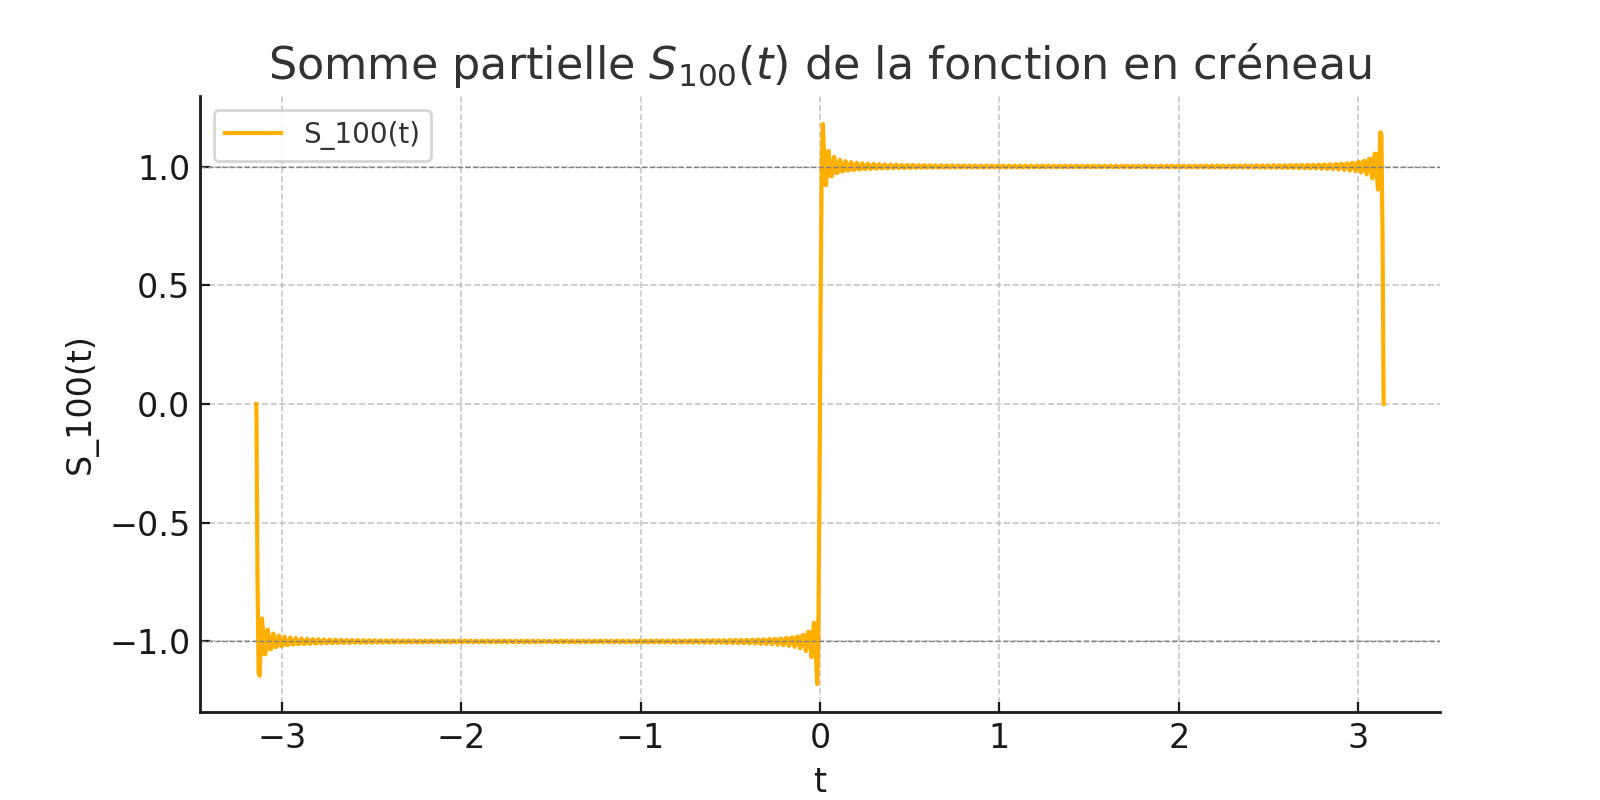
\includegraphics[width=\linewidth]{S_p_t_100.png}
    \caption{Somme partielle \( S_{100}(t) \)}
\end{minipage}
\end{figure}

\vspace{0.5em}
\noindent\textbf{Code utilisé} : \hyperref[annexe_code_py]{voir annexe}



\section{Conclusion}

À travers ce projet, nous avons étudié en détail le phénomène de Gibbs, qui se manifeste lors de l’approximation d’une fonction périodique discontinue par sa série de Fourier. Bien que cette série converge ponctuellement en tout point, elle ne converge pas uniformément près des discontinuités : les sommes partielles dépassent la valeur réelle de la fonction, et ce dépassement ne disparaît jamais, même si on ajoute de plus en plus de termes.

Ce phénomène nous montre que la convergence d'une série de Fourier dépend fortement de la régularité de la fonction : pour les fonctions continues, la convergence est uniforme ; pour les fonctions discontinues, elle peut provoquer des artefacts comme le dépassement observé.

L’étude du phénomène de Gibbs est importante en mathématiques, car elle souligne une limite des séries de Fourier. Elle invite à réfléchir sur les notions de convergence (ponctuelle, uniforme), sur les effets des discontinuités, et sur les choix des méthodes d’approximation selon le type de fonction.

On retrouve ce type de comportement dans d'autres domaines mathématiques : par exemple, lorsqu’on approxime une fonction à variation rapide par des polynômes ou par d’autres séries orthogonales, des oscillations peuvent également apparaître aux endroits où la fonction change brusquement.

Ce projet nous a permis d’approfondir des outils fondamentaux de l’analyse comme les intégrales, les séries trigonométriques, et l’étude des dérivées et des variations. Il montre comment une idée simple — approximer une fonction par des sinus et cosinus — peut mener à des phénomènes subtils et profonds.



\appendix
\section{Annexe :}


\label{annexe_code_continue}


\subsection{Fonction continue : $f(x) = 1 + \sin(x)$}

Le code suivant permet de tracer la fonction continue \( f(x) = 1 + \sin(x) \) ainsi que ses premières sommes partielles de Fourier. On observe que, dans ce cas, la convergence est uniforme sur \( \mathbb{R} \) sans phénomène de dépassement.

\begin{minted}[fontsize=\small, linenos]{python}
import numpy as np
import matplotlib.pyplot as plt

def f(x):
    return 1 + np.sin(x)

def S_N(x, N):
    if N == 0:
        return np.ones_like(x)
    else:
        return 1 + np.sin(x)

x = np.linspace(-np.pi, np.pi, 1000)

plt.figure(figsize=(10, 6))
plt.plot(x, f(x), label="f(x) = 1 + sin(x)", color='black', linewidth=2)
plt.plot(x, S_N(x, 0), label="S₀(x) = 1", linestyle='--', color='red')
plt.plot(x, S_N(x, 1), label="S₁(x) = 1 + sin(x)", linestyle='--', color='blue')

plt.title("Séries de Fourier partielles de f(x) = 1 + sin(x)")
plt.xlabel("x")
plt.ylabel("f(x) et S_N(x)")
plt.axhline(0, color='gray', linewidth=0.5)
plt.axvline(0, color='gray', linewidth=0.5)
plt.legend()
plt.grid(True)
plt.show()
\end{minted}


\label{annexe_code_python}
\subsection{Fonction discontinue : Fonction porte}

\begin{minted}[fontsize=\small, linenos]{python}
import numpy as np
import matplotlib.pyplot as plt

# Fonction pour calculer la somme partielle de Fourier
def f_partielle(x, N):
    s = np.full_like(x, 0.5)
    for n in range(1, N + 1):
        coef = (2 / (n * np.pi)) * np.sin(n * np.pi / 2)
        s += coef * np.cos(n * x)
    return s


x = np.linspace(-np.pi, np.pi, 1000)
f_exact = np.where(np.abs(x) < np.pi / 2, 1, 0)

# Tracés pour plusieurs N
for N in [1, 5, 10, 100]:
    plt.figure(figsize=(8, 4))
    plt.plot(x, f_partielle(x, N), label=f"S_{N}(x)")
    plt.plot(x, f_exact, 'k--', label='f(x)', linewidth=1)
    plt.title(f"Série de Fourier partielle pour N = {N}")
    plt.xlabel("x")
    plt.ylabel(f"S_{N}(x)")
    plt.legend()
    plt.grid(True)
    plt.tight_layout()
    plt.savefig(f"serie_fourier_N{N}.png")
    plt.show()
\end{minted}



\label{annexe_code_py}
\subsection{Les courbes de \( S_p(t) \)}

Le code suivant permet de tracer les sommes partielles \( S_p(t) \) de la série de Fourier de la fonction étudiée dans la partie théorique pour plusieurs valeurs de \( p \) (5, 10, 50, 100). Ces courbes illustrent l’apparition du phénomène de Gibbs.

\begin{minted}[fontsize=\small, linenos]{python}
import numpy as np
import matplotlib.pyplot as plt

# Définition de la somme partielle S_p(t)
def S_p(t, p):
    result = np.zeros_like(t)
    for k in range(1, p + 1):
        result += np.sin((2 * k - 1) * t) / (2 * k - 1)
    return (4 / np.pi) * result


t_vals = np.linspace(-np.pi, np.pi, 1000)


for p in [5, 10, 50, 100]:
    plt.figure(figsize=(8, 4))
    plt.plot(t_vals, S_p(t_vals, p), label=f"S_{p}(t)")
    plt.axhline(1, color='gray', linestyle='--', linewidth=0.5)
    plt.axhline(-1, color='gray', linestyle='--', linewidth=0.5)
    plt.title(f"Série de Fourier partielle pour p = {p}")
    plt.xlabel("t")
    plt.ylabel(f"S_{p}(t)")
    plt.grid(True)
    plt.legend()
    plt.tight_layout()
    plt.savefig(f"S_p_t_{p}.png")
    plt.show()
\end{minted}


\end{document}









